\documentclass[border=10pt]{standalone}
\usepackage{tikz}

%Provide default strings for packet field descriptions in english if anything else not set
\providecommand{\tstrsep}{Separator}
\providecommand{\tstrdata}{Data}

\usetikzlibrary{positioning,arrows,decorations.pathreplacing}

\begin{document}
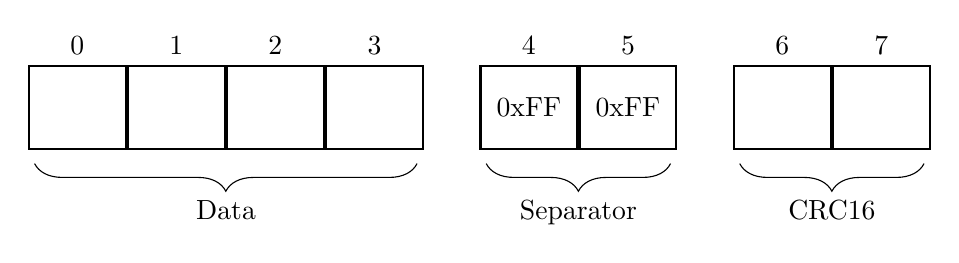
\begin{tikzpicture}[node distance=0pt,minimum size=1pt,auto]

\tikzstyle{pfield}=[rectangle,minimum width=35pt,minimum height=30pt,draw=black,thick];

\node [pfield,label={0}] (b0) {};
\node [pfield,label={1}] (b1) [right= of b0.east] {};
\node [pfield,label={2}] (b2) [right= of b1.east] {};
\node [pfield,label={3}] (b3) [right= of b2.east] {};
\node [pfield,label={4}] (b4) [right= of b3.east,xshift=20pt] {0xFF};
\node [pfield,label={5}] (b5) [right= of b4.east] {0xFF};
\node [pfield,label={6}] (b6) [right= of b5.east,xshift=20pt] {};
\node [pfield,label={7}] (b7) [right= of b6.east] {};

\draw [decorate,decoration={brace,amplitude=10pt,raise=5pt}] (b3.315) -- (b0.225) node [black,midway,align=center,yshift=-15pt] {\tstrdata};

\draw [decorate,decoration={brace,amplitude=10pt,raise=5pt}] (b5.315) -- (b4.225) node (t0) [black,midway,align=center,yshift=-15pt] {\tstrsep};

\draw [decorate,decoration={brace,amplitude=10pt,raise=5pt}] (b7.315) -- (b6.225) node (t0) [black,midway,align=center,yshift=-15pt] {CRC16};

\end{tikzpicture}
\end{document}